\documentclass[a4paper,10pt,notitlepage]{scrreprt}

\usepackage[T1]{fontenc}
\usepackage[english]{babel}
\usepackage[utf8x]{inputenc}
\usepackage{setspace}
\usepackage{subfig}
\usepackage{textcomp}
\usepackage{graphicx}
\usepackage{fixltx2e}
\usepackage{multirow}
\usepackage{array}
\usepackage{amssymb}
\usepackage{amsmath}
\usepackage{subfig}
\usepackage{nomencl}
\usepackage[pdfborder={0 0 0}]{hyperref}
\usepackage{natbib}
% \usepackage{makeidx}
\usepackage{nicefrac}
\usepackage{bbold}

\captionsetup{labelfont=footnotesize,textfont=footnotesize}

\newcolumntype{x}[1]{>{\begin{flushleft}$}p{#1}<{$\end{flushleft}}}
\newcolumntype{y}[1]{>{\begin{center}$}p{#1}<{$\end{center}}}
\newcolumntype{z}[1]{>{\begin{flushright}$}p{#1}<{$\end{flushright}}}
\newcolumntype{m}{>{$}l<{$}}
\newcolumntype{n}{>{$}c<{$}}
\newcolumntype{o}{>{$}r<{$}}

\newcommand{\mat}[1]{\mathbf{#1}} 

\bibliographystyle{plain}

% Title Page
\title{Scientific Visualization\\Project III}
\author{Milian Wolff}


\begin{document}
\maketitle

\begin{abstract}
During the third project for the the scientific visualization class by Eugene
Zhang we got an introduction to vector calculus and vector field design. We
investigate the topology of vector fields and write a JavaView based
application for LIC-based vector field design and visualization.

The source code of my exercise solutions can be found online under

\begin{center}\url{https://github.com/milianw/scivi}\end{center}
\end{abstract}

\begingroup
\let\clearpage\relax

\tableofcontents
\endgroup

\chapter{Vector Field Design}

The vector field design application is based on JavaView which already has
built-in LIC visualization support. As such, this task was quite easy.

In my implementation, the user picks a type of design element (see below) he
wants to add to the vector field. Then he can add such a feature to the vector
field by clicking into the vector field domain. Existing features can be
removed, altered and moved via drag'n'drop. The view gets updated automatically.

\section{Design Elements}

I have decided to implement the following design elements based on the
equations given in the recitation:

\begin{itemize}
 \item constant, fig \ref{fig:constant}: $\vec{V}_i(\vec{r}) = \sigma
\vec{e}_i$, with $\vec{e}_i$ being a normalized direction vector
 \item generic, fig \ref{fig:generic}: $\vec{V}_i(\vec{r}) = \sigma \mat{A}
(\vec{r} - \vec{r}_i) $, with $\mat{A}$ being an arbitrary $2\times2$~matrix
 \item sink, fig. \ref{fig:sink}: generic with diagonal $\mat{A}$ and entries
$-1$
 \item source, fig \ref{fig:source}: generic with diagonal $\mat{A}$ and
entries $1$
 \item saddle, fig \ref{fig:saddle}: generic with diagonal $\mat{A}$ and
entries $1$ and $-1$
 \item focus, fig \ref{fig:focus}: generic with $\mat{A} = \left(
\begin{array}{cc}
\cos(\theta) & -\sin(\theta) \\
\sin(\theta) & \cos(\theta) \end{array} \right)$
 \item center, clockwise, fig \ref{fig:center-cw}: generic with $\mat{A} =
\left(
\begin{array}{cc}
0 & 1 \\
-1 & 0 \end{array} \right)$
 \item center, counter-clockwise, fig \ref{fig:center-cc}: generic with $\mat{A}
= \left(
\begin{array}{cc}
0 & -1 \\
1 & 0 \end{array} \right)$
 \item converging, fig \ref{fig:converging}: $\sigma (\vec{e}_i + ((\vec{r} -
\vec{r}_i) \cdot \vec{n}_i) \vec{n}_i$, with $\vec{e}_i$ being a normalized
direction vector and $\vec{n}_i$ the normal to that
 \item diverging, fig \ref{fig:diverging}: like the converging element
multiplied by $-1$
\end{itemize}

In the equations above, $\sigma$ is the scaling factor

\begin{equation}
 \sigma = s \exp(-d |\vec{r}_i - \vec{r}|^2),
\end{equation}

with $s$ denoting the strength and $\vec{r}_i$ being the base point of the
design element, i.e. the point where the user clicked.

\begin{figure}
  \centering
  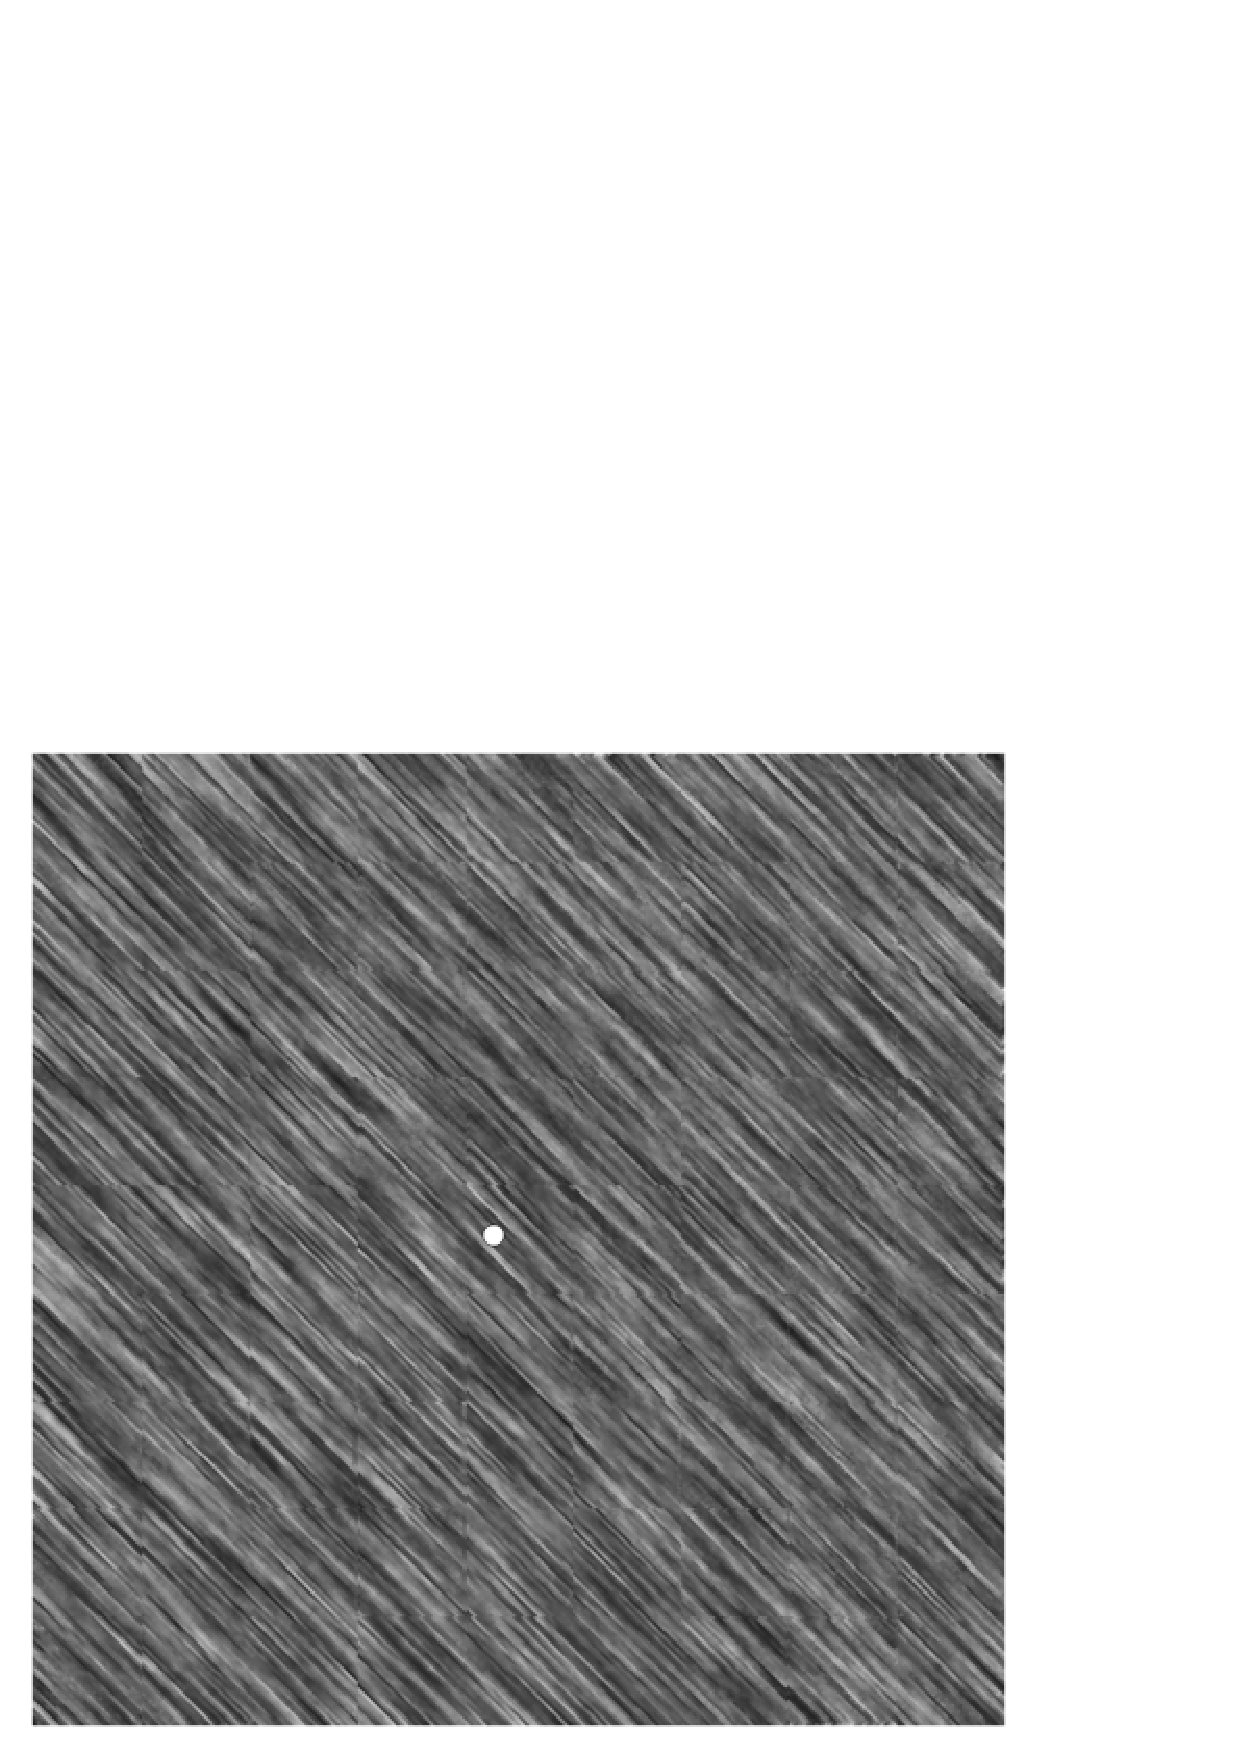
\includegraphics[scale=0.5]{img-3-2/constant.png}
  \caption{constant vector field design element}
  \label{fig:constant}
\end{figure}

\begin{figure}
  \centering
  \includegraphics[scale=0.5]{img-3-2/generic.png}
  \caption{generic vector field design element}
  \label{fig:generic}
\end{figure}

\begin{figure}
  \centering
  \includegraphics[scale=0.5]{img-3-2/sink.png}
  \caption{sink vector field design element}
  \label{fig:sink}
\end{figure}

\begin{figure}
  \centering
  \includegraphics[scale=0.5]{img-3-2/source.png}
  \caption{source vector field design element}
  \label{fig:source}
\end{figure}

\begin{figure}
  \centering
  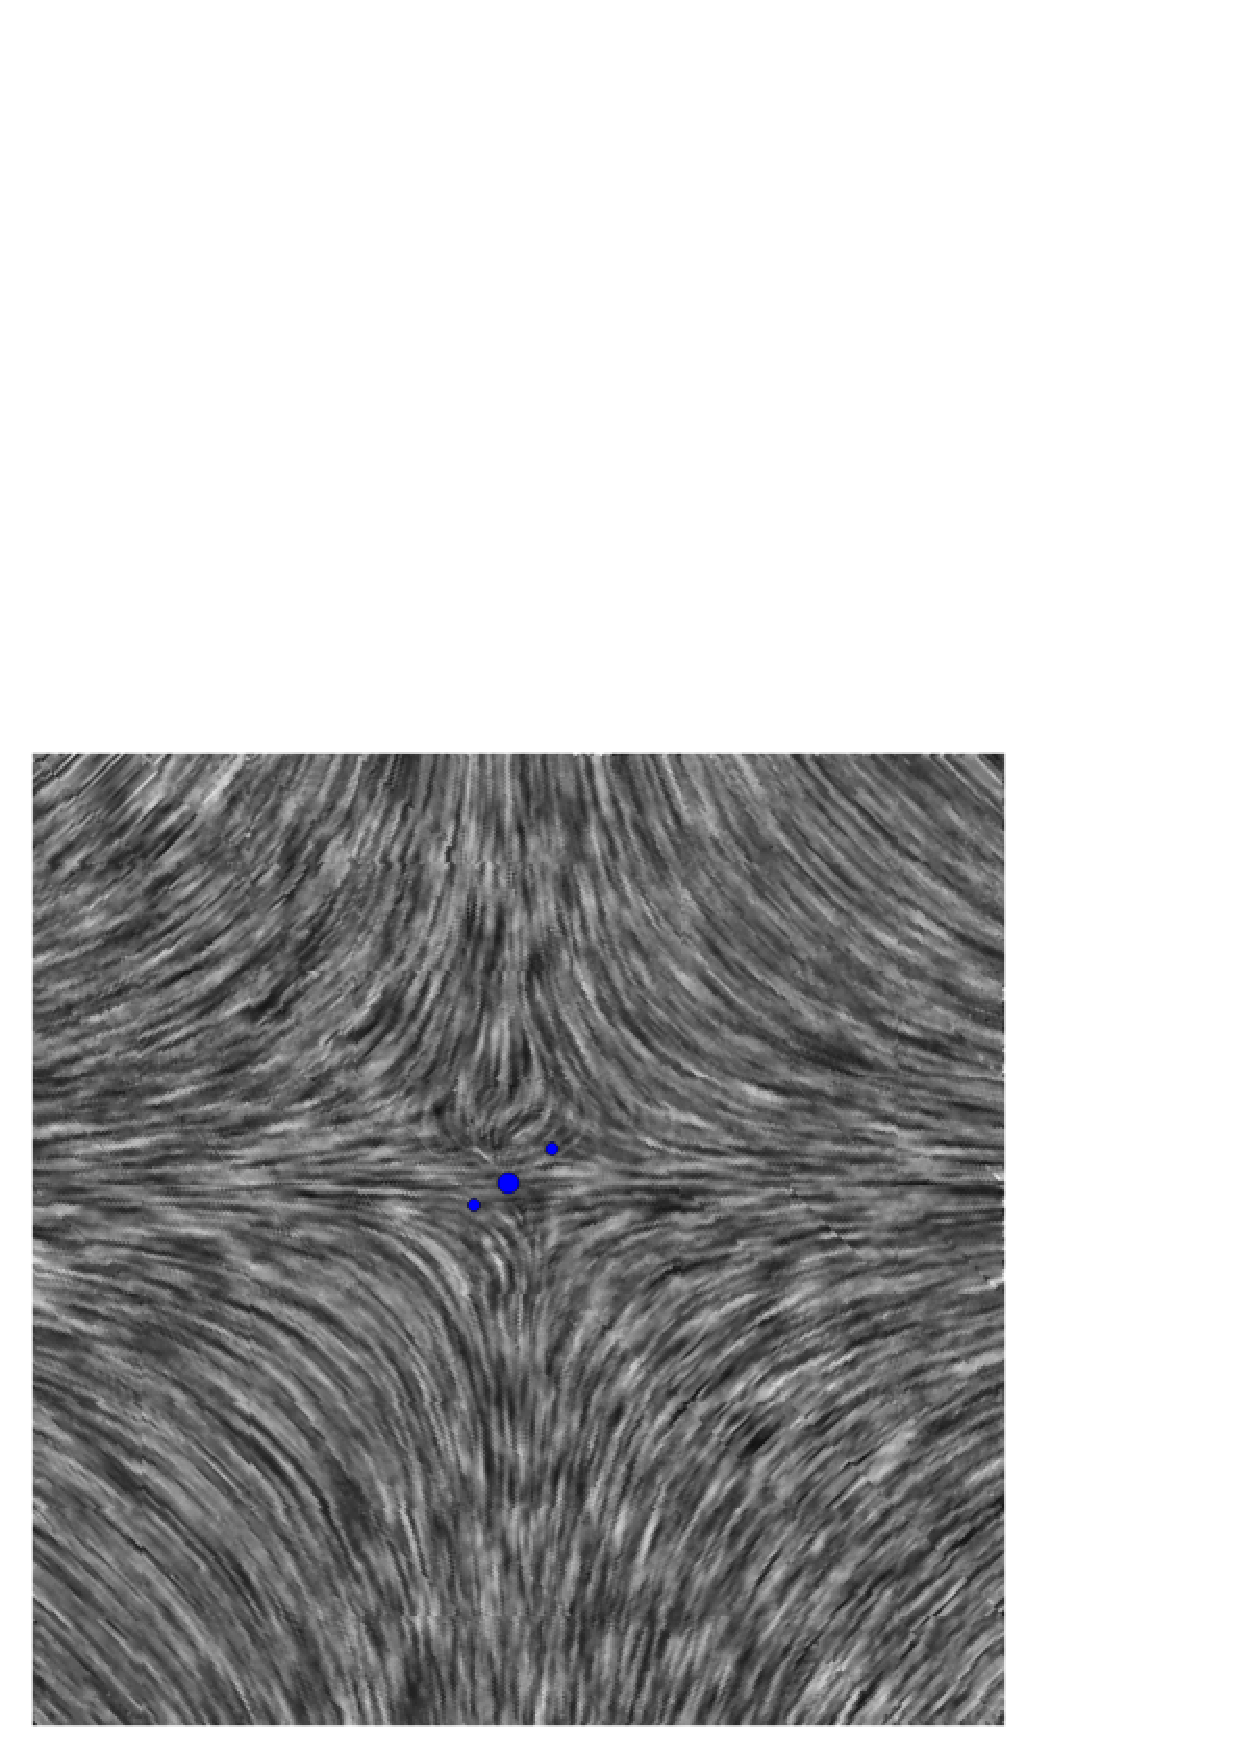
\includegraphics[scale=0.5]{img-3-2/saddle.png}
  \caption{saddle vector field design element}
  \label{fig:saddle}
\end{figure}

\begin{figure}
  \centering
  \includegraphics[scale=0.5]{img-3-2/focus.png}
  \caption{focus vector field design element}
  \label{fig:focus}
\end{figure}

\begin{figure}
  \centering
  \includegraphics[scale=0.5]{img-3-2/center-cw.png}
  \caption{clockwise center vector field design element}
  \label{fig:center-cw}
\end{figure}

\begin{figure}
  \centering
  \includegraphics[scale=0.5]{img-3-2/center-cc.png}
  \caption{counter-clockwise center vector field design element}
  \label{fig:center-cc}
\end{figure}

\begin{figure}
  \centering
  \includegraphics[scale=0.5]{img-3-2/converging.png}
  \caption{converging vector field design element}
  \label{fig:converging}
\end{figure}

\begin{figure}
  \centering
  \includegraphics[scale=0.5]{img-3-2/diverging.png}
  \caption{diverging vector field design element}
  \label{fig:diverging}
\end{figure}

\section{Flow Rotation}

The flow can easily rotated by an arbitrary angle $\theta$ via
matrix-multiplication of each vector in the discretized domain with a rotation
matrix:

\begin{equation}
 \vec{v}'(\vec{r}) = \mat{R} \vec{v}(\vec{r})
\end{equation}

The rotation matrix is given by

\begin{equation}
 \mat{R} = \left(
\begin{array}{cc}
\cos(\theta) & -\sin(\theta) \\
\sin(\theta) & \cos(\theta) \end{array} \right)
\end{equation}

An example can be seen in fig. \ref{fig:flow-rotation}.

\begin{figure}
  \centering
  \subfloat[basis]{
    \includegraphics[scale=0.5]{img-3-2/rotate-a.png}}
  \\
  \subfloat[rotated]{
    \includegraphics[scale=0.5]{img-3-2/rotate-b.png}}
  \caption{flow rotation}
  \label{fig:flow-rotation}
\end{figure}

\section{Flow Reflection}

Similar to above, flow reflection is achieved via matrix multiplication. In my
implementation, reflection can be turned on and off and is supposed to be used
in combination with flow rotation. When flow reflection is turned on, the sign
of the second column in the rotation matrix changes sign:

\begin{equation}
 \mat{R}' = \mat{R} \cdot \left( \begin{array}{c} 1 \\ -1\end{array} \right)
\end{equation}

An example for flow reflection is shown in fig. \ref{fig:flow-reflection}.

\begin{figure}
  \centering
  \subfloat[basis]{
    \includegraphics[scale=0.5]{img-3-2/reflect-a.png}}
  \\
  \subfloat[reflected]{
    \includegraphics[scale=0.5]{img-3-2/reflect-b.png}}
  \caption{flow reflection}
  \label{fig:flow-reflection}
\end{figure}

\end{document}

% kate: replace-tabs on;